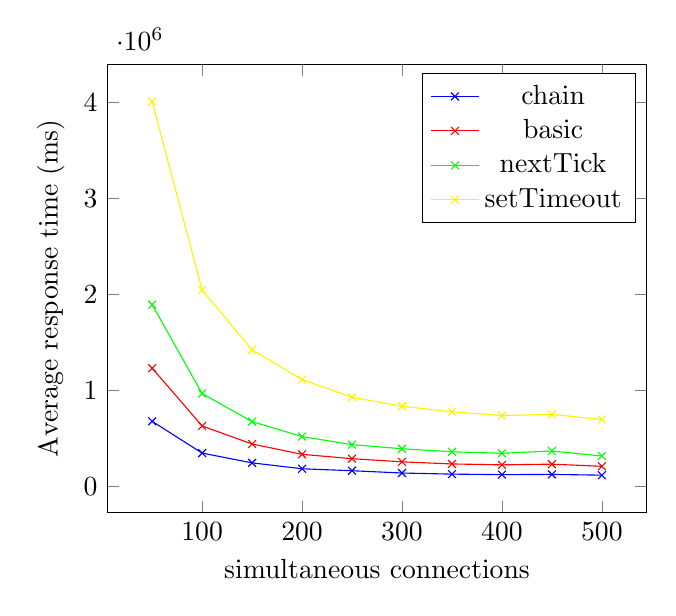
\begin{tikzpicture}
\begin{axis}[ylabel=Average response time (ms), xlabel=simultaneous connections]
\addplot[color=blue, mark=x] coordinates {(500,114995.32528) (450,122838.59306666667) (400,120520.87927) (350,125804.85788) (300,137353.90422666667) (250,161158.845064) (200,181766.47594) (150,243137.08273333334) (100,345101.4) (50,676236.53308) };
\addplot[color=red, mark=x] coordinates {(500,207373.03734) (450,229747.1160977778) (400,222559.42405) (350,231843.3596857143) (300,253938.66218) (250,286722.145072) (200,332173.43176) (150,439872.5621466667) (100,627831.77992) (50,1230640.684) };
\addplot[color=green, mark=x] coordinates {(500,314416.82756) (450,366918.21844) (400,343154.9846) (350,358588.17509142857) (300,390450.68483333336) (250,433312.381768) (200,517243.12997) (150,673192.3322) (100,965474.43368) (50,1892591.87264) };
\addplot[color=yellow, mark=x] coordinates {(500,695165.448196) (450,749051.9985422222) (400,736351.59995) (350,775751.00084) (300,833511.3019933334) (250,927298.448824) (200,1111177.58162) (150,1421107.2465333333) (100,2045025.33614) (50,4009760.531) };
\legend{chain, basic, nextTick, setTimeout}
\end{axis}
\end{tikzpicture}
